\documentclass[a4paper,12pt]{article}
\usepackage[utf8]{inputenc}
\usepackage[T1]{fontenc}
\usepackage[czech,english]{babel}
\usepackage{graphicx}
\usepackage{hyperref}
\usepackage{geometry}
\usepackage{xcolor}
\usepackage{float}
\usepackage{mdframed}
\usepackage{amsmath}
\geometry{margin=2.5cm}

\setlength{\parskip}{0.8em}
\setlength{\parindent}{0pt}

\begin{document}
	
	\begin{center}
		{\Large \textbf{BPA-KOM Lab 5 - DHCP}}\\[1em]
	\end{center}
	
	\vspace{1cm}
	
	\begin{center}
		\begin{tabular}{|c|c|}
			\hline
			\textbf{Name} & Dave Galea \\ \hline
			\textbf{VUT ID} & 284844 \\ \hline
			\textbf{Lab Number} & 5 \\ \hline
			\textbf{Date} & December 2025 \\ \hline
		\end{tabular}
	\end{center}
	
	\vspace{0.5cm}
	\hrule
	\vspace{0.5cm}
	
	\section*{1. Objective 1}
	
	\textbf{Task Assignment:} The aim of this task was to release and renew IP configuration via DHCP and capture communication with the DHCP server in Wireshark.
	
	\textbf{Solution:}\\[1em]
	NOTE: for the wireshark portion of this lab, WIFI was used instead of Ethernet, as the lab was performed in an area without ethernet availability. This did not hinder in analyzing the DHCP process.
	
	First, DHCP ip address assignment was confirmed to be true on the pc used for this lab. This is the case, as shown below.
	\begin{figure}[H]
		\centering
		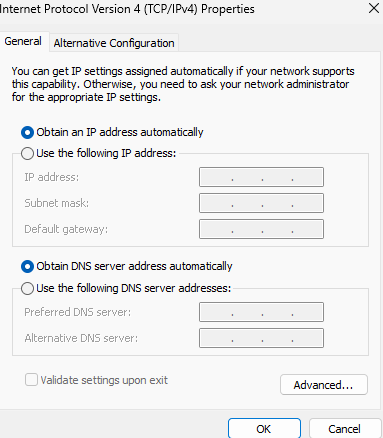
\includegraphics[width=\linewidth, height=0.4\textheight, keepaspectratio]{photos/1-1}
		\caption{Pc using DHCP IP address assignment.}
	\end{figure}
	
	Then, after packets started being captured in Wireshark, in CMD, the current configuration of the Wifi interface was displayed:
	\begin{figure}[H]
		\centering
		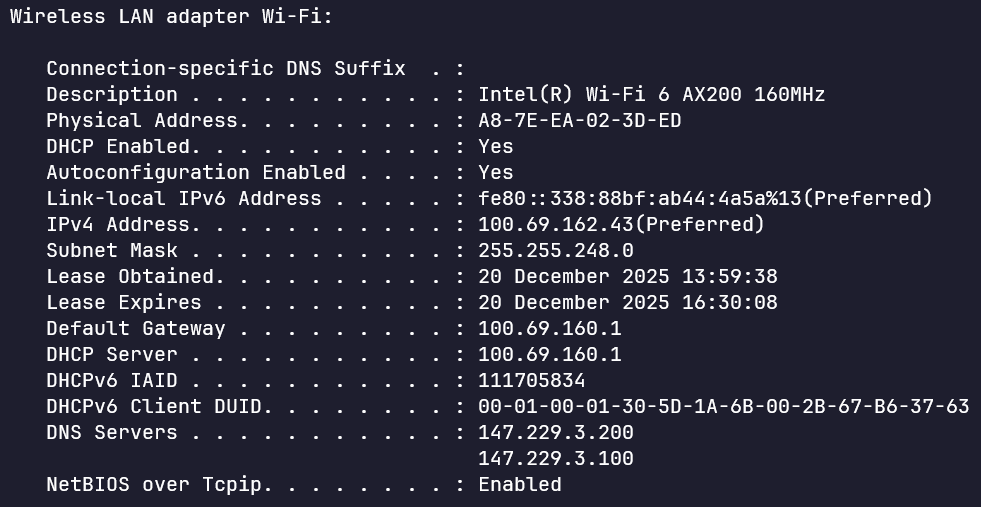
\includegraphics[width=\linewidth, height=0.4\textheight, keepaspectratio]{photos/1-3}
		\caption{Current configuration of the Wifi interface.}
	\end{figure}
	
	Then, following the commands \texttt{ipconfig /release} and \texttt{ipconfig /renew}, the configuration was displayed once again. It should be noted that the IP address assigned remained the same, this is be cause the DHCP server keeps a binding table: it remembers which IP was assigned to which MAC address.
	\begin{figure}[H]
		\centering
		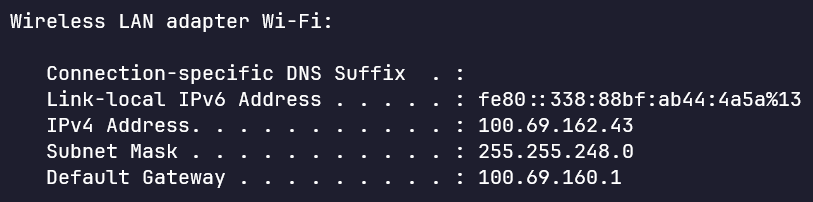
\includegraphics[width=\linewidth, height=0.4\textheight, keepaspectratio]{photos/1-5}
		\caption{Configuration following appropriate CMD commands.}
	\end{figure}
	
	Then in Wireshark, packets stopped being captured.

	
	\vspace{1em}
	\hrule
	\vspace{0.5em}
	
	\section*{2. Objective 2}
	
	\textbf{Task Assignment:} The aim of this task was to analyse DHCP packet content during communication states.
	
	\textbf{Solution:}\\[1em]
	After setting the appropriate filter to show captured DHCP packets in wireshark, the following was shown:
	\begin{figure}[H]
		\centering
		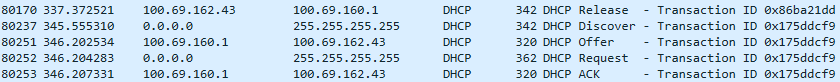
\includegraphics[width=\linewidth, height=0.4\textheight, keepaspectratio]{photos/2-1}
		\caption{Captured DHCP packets in Wireshark.}
	\end{figure}
	
	
	The first packet is the DHCP release message. The Dynamic Host Configuration Protocol section was unrolled, and displayed as follows:
	\begin{figure}[H]
		\centering
		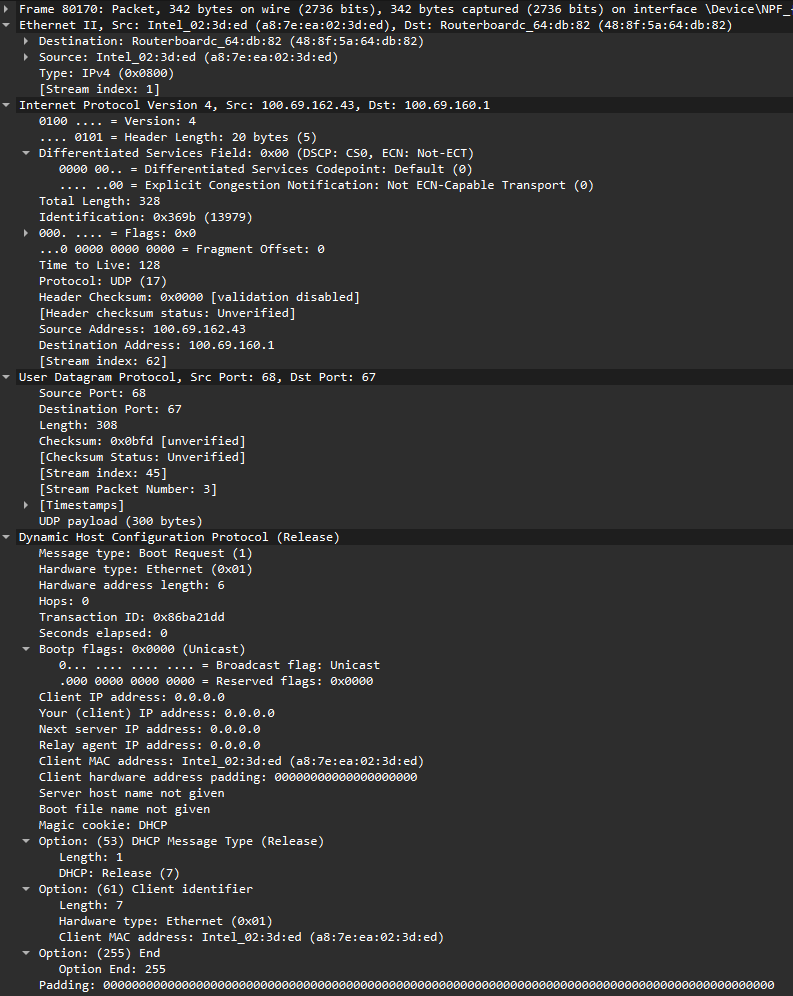
\includegraphics[width=\linewidth, height=0.55\textheight, keepaspectratio]{photos/2-2}
		\caption{DHCP release message.}
	\end{figure}
	From the above, the following can be noted:
	\begin{itemize}
		\item Message type: Boot Request
		\item Client Physical address: a8:7e:ea:02:3d:ed
		\item Client Logical addresses: 0.0.0.0
		\item Numeric value of DHCP release message type: 7
		\item Source port: 68
		\item Destination port: 67
		\item Destination IP address: 100.69.160.1
		\item Destination MAC address: 48:8f:5a:64:db:82
	\end{itemize}
	
	
	The second packet is the DHCP discover message. The Dynamic Host Configuration Protocol section was unrolled, and displayed as follows:
	\begin{figure}[H]
		\centering
		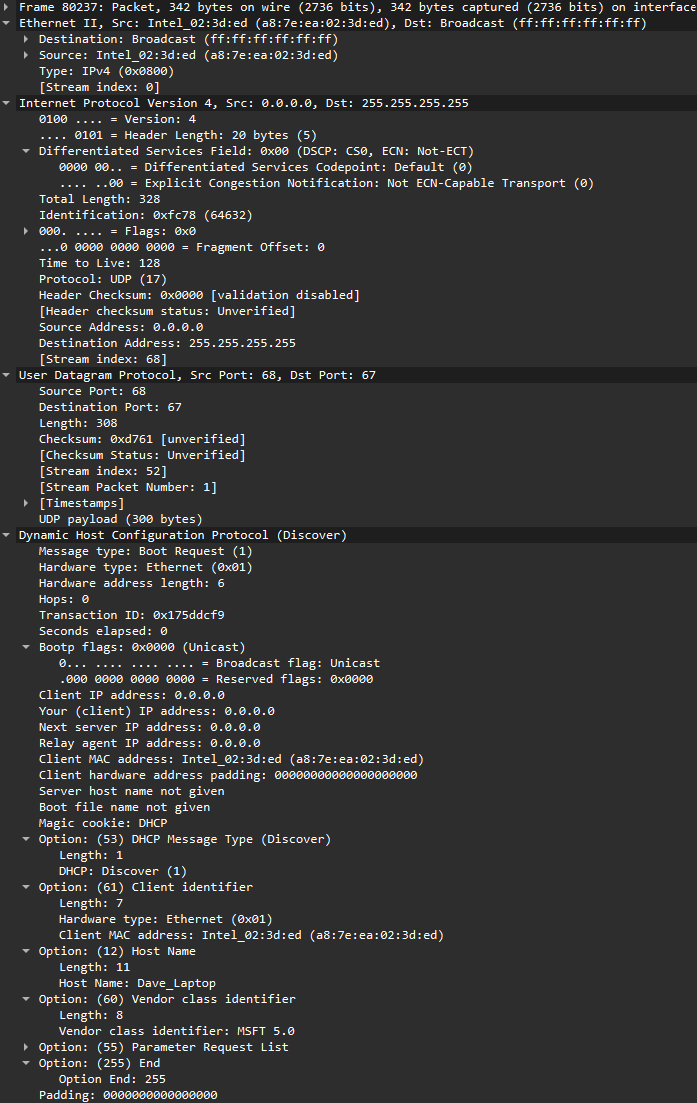
\includegraphics[width=\linewidth, height=0.55\textheight, keepaspectratio]{photos/2-3}
		\caption{DHCP discover message.}
	\end{figure}
	From the above, the following can be noted:
	\begin{itemize}
		\item Message type: Boot Request
		\item Client Logical addresses: 0.0.0.0
		\item DHCP server Identifier: No, because client doesn't yet know which server to reference
		\item Source port: 68
		\item Destination port: 67
		\item Destination IP address: 255.255.255.255
		\item Destination MAC address: ff:ff:ff:ff:ff:ff
	\end{itemize}
	
	
	The third packet is the DHCP offer message. The Dynamic Host Configuration Protocol section was unrolled, and displayed as follows:
	\begin{figure}[H]
		\centering
		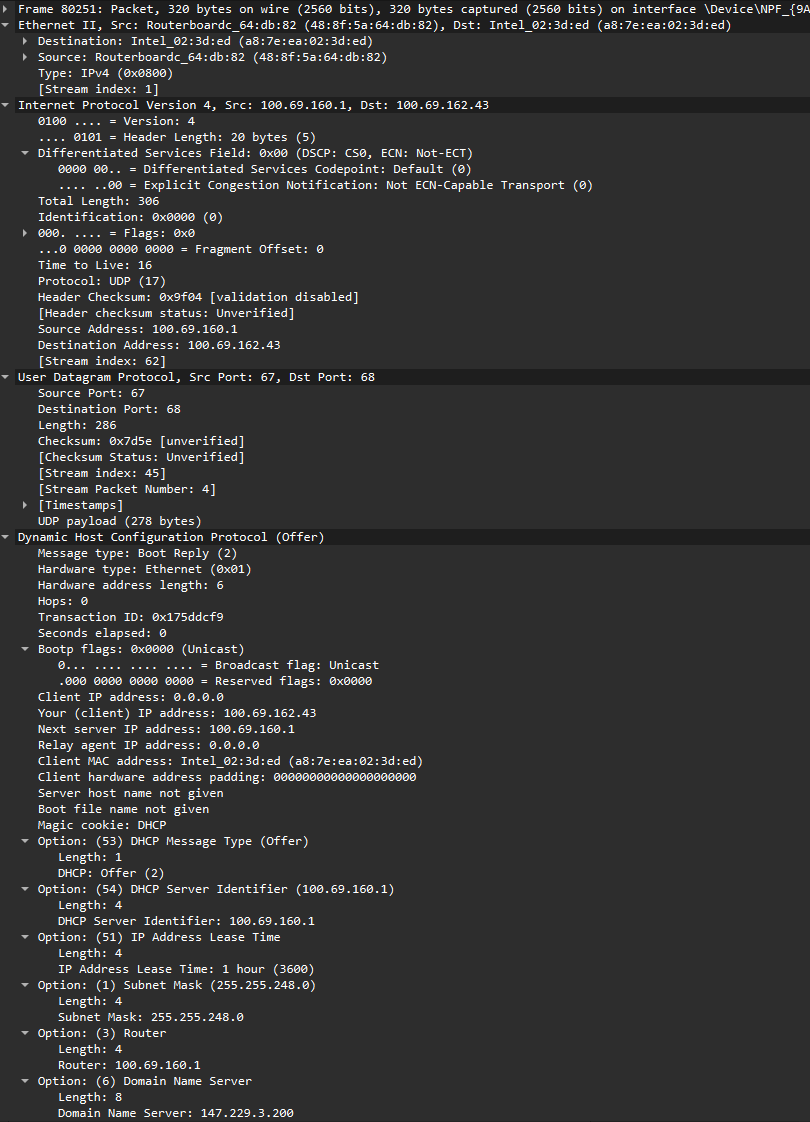
\includegraphics[width=\linewidth, height=0.55\textheight, keepaspectratio]{photos/2-4}
		\caption{DHCP offer message.}
	\end{figure}
	From the above, the following can be noted:
	\begin{itemize}
		\item Message type: Boot Reply
		\item IP address lease time: 1 hour
		\item Option Parameters: 53, 54, 51, 1, 3, 6
		\item Numeric value of DHCP release message type: 7
		\item Source port: 67
		\item Destination port: 68
		\item Destination IP address: 100.69.162.43
		\item Destination MAC address: a8:7e:ea:02:3d:ed
	\end{itemize}
	
	
	The fourth packet is the DHCP request message. The Dynamic Host Configuration Protocol section was unrolled, and displayed as follows:
	\begin{figure}[H]
		\centering
		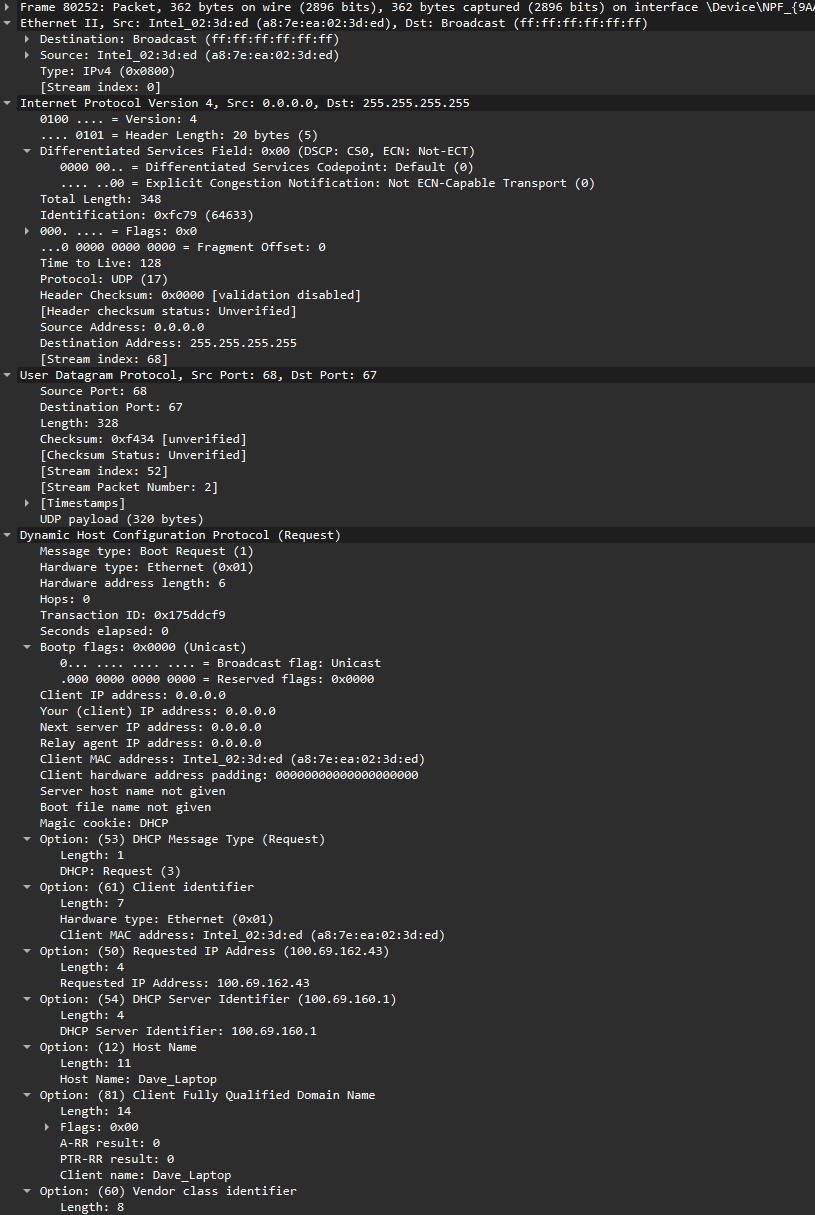
\includegraphics[width=\linewidth, height=0.55\textheight, keepaspectratio]{photos/2-5}
		\caption{DHCP request message.}
	\end{figure}
	From the above, the following can be noted:
	\begin{itemize}
		\item Message type: Boot Request
		\item IP address specified in options fields: Requested (100.69.162.43), Server Identifier (100.69.160.1)
		\item Source port: 68
		\item Destination port: 67
		\item Destination IP address: 255.255.255.255
		\item Destination MAC address: ff:ff:ff:ff:ff:ff
	\end{itemize}
	
	
	The fifth packet is the DHCP ACK message. The Dynamic Host Configuration Protocol section was unrolled, and displayed as follows:
	\begin{figure}[H]
		\centering
		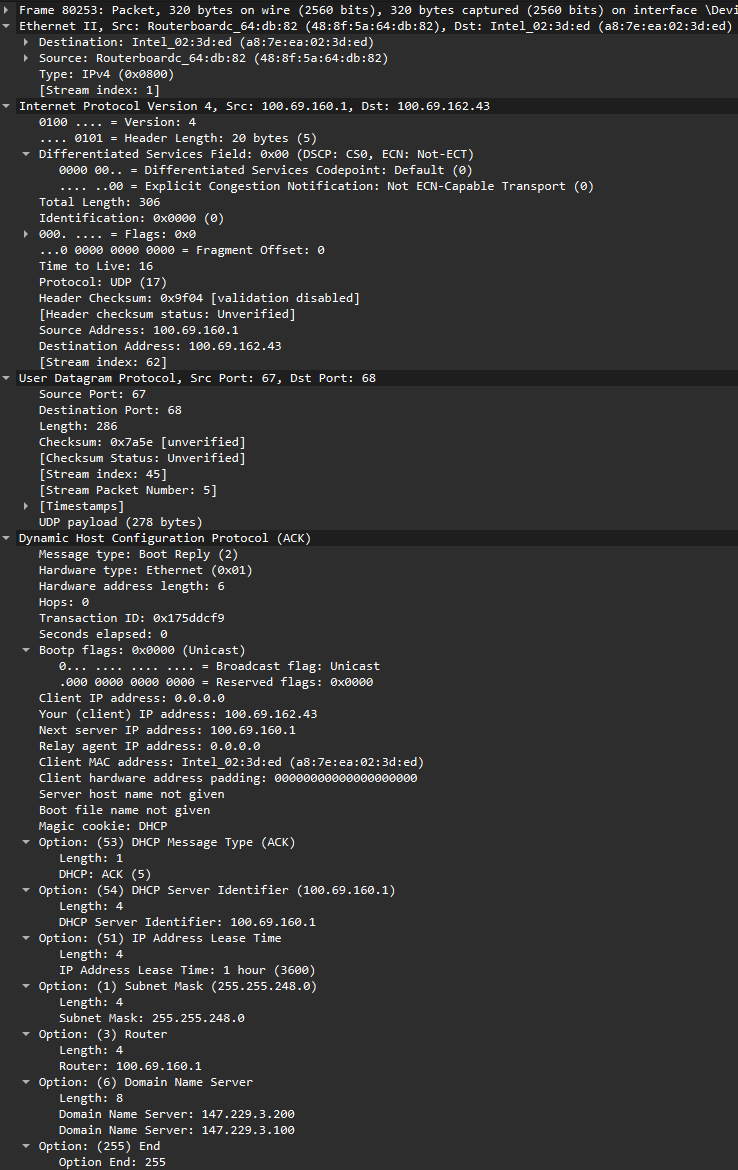
\includegraphics[width=\linewidth, height=0.55\textheight, keepaspectratio]{photos/2-6}
		\caption{DHCP ACK message.}
	\end{figure}
	From the above, the following can be noted:
	\begin{itemize}
		\item Message type: Boot Reply
		\item Changes with offer message: Destination IP address, source port, destination port.
		\item Source port: 68
		\item Destination port: 67
		\item Destination IP address: 100.69.162.43
		\item Destination MAC address: a8:7e:ea:02:3d:ed
	\end{itemize}
	Throughout the entire communication, it can be noted that the transaction ID was the same for all messages besides for the release message. For the release message, transaction ID was 0x86ba21dd, while for the rest it was 0x175ddcf9.
	
	
	\vspace{1em}
	\hrule
	\vspace{0.5em}
	
	\section*{3. Objective 3}
	
	\textbf{Task Assignment:} The aim of this task was to generate graphs from the captured communication.
	
	\textbf{Solution:} \\ [1em]
	From the Wireshark graph generation software, the graphs for the packets and bytes sent during the DHCP communication were generated: 
	\begin{figure}[H]
		\centering
		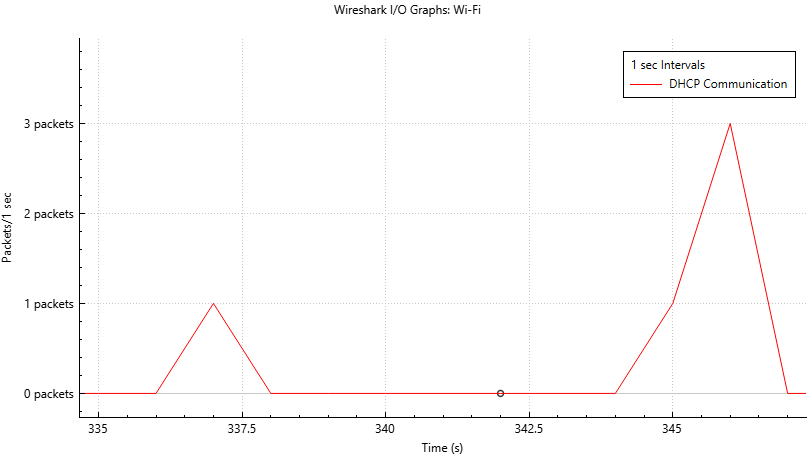
\includegraphics[width=\linewidth, height=0.55\textheight, keepaspectratio]{photos/3-2}
		\caption{Packets sent during the DHCP communication.}
	\end{figure}
	
	\begin{figure}[H]
		\centering
		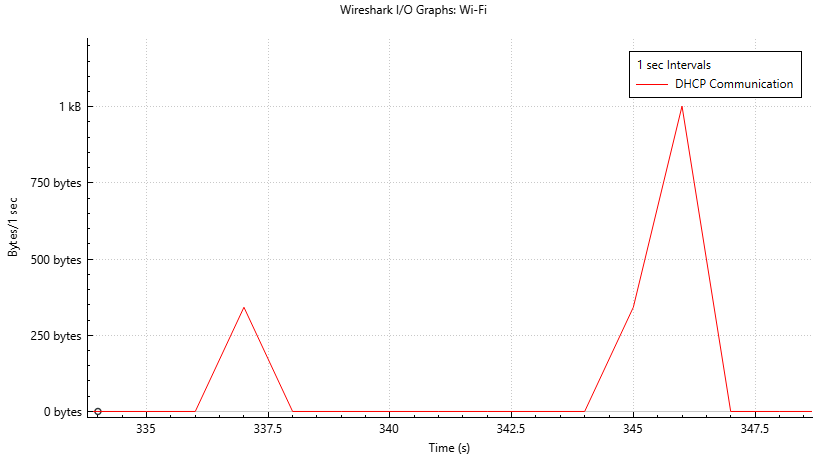
\includegraphics[width=\linewidth, height=0.3\textheight, keepaspectratio]{photos/3-3}
		\caption{Bytes sent during the DHCP communication.}
	\end{figure}

	\vspace{1em}
	\hrule
	\vspace{0.5em}
	
	\section*{4. Objective 4}
	
	\textbf{Task Assignment:} The aim of this task was to create the topology in Cisco Packet Tracer.
	
	\textbf{Solution:} \\ [1em]
	After adding the necessary components specified in the lab, the topology for the rest of the lab is as follows:
	\begin{figure}[H]
		\centering
		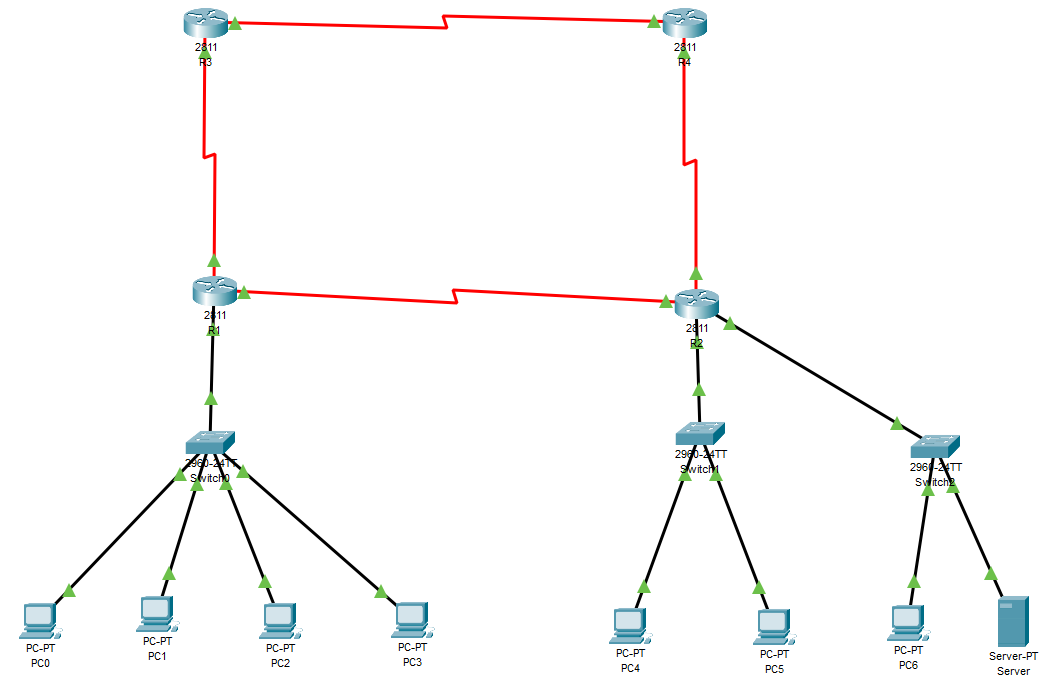
\includegraphics[width=\linewidth, height=0.3\textheight, keepaspectratio]{photos/4-4}
		\caption{Topology in Cisco Packet Tracer.}
	\end{figure}
	
	After setting the topology, connectivity was verified from the PCs:
	\begin{figure}[H]
		\centering
		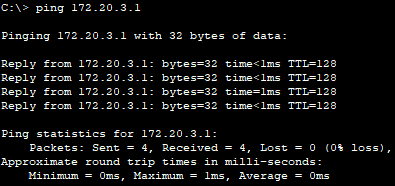
\includegraphics[width=\linewidth, height=0.3\textheight, keepaspectratio]{photos/4-5}
		\caption{Verifying connectivity with ping.}
	\end{figure}
	
	
	\vspace{1em}
	\hrule
	\vspace{0.5em}
	
	\section*{5. Objective 5}
	
	\textbf{Task Assignment:} The aim of this task was to configure R2 as the DHCP server for both connected LANs. Additionally, PCs were set to use DHCP and analyse communication.
	
	\textbf{Solution:}\\[1em]
	Setting R2 as the DHCP server for both connected LANs involved defining two pools on the router, one for the LAN with \texttt{172.20.1/24} address space and one for \texttt{172.20.3.0/24} address space.
	
	First, the addresses which shouldn't be assigned by the DHCP server are explicitly defined. In total, 12 total addresses are excluded by using the following commands:
	\begin{itemize}
		\item \texttt{R2(config)\#ip dhcp excluded-address 172.20.1.254} 
		\item \texttt{R2(config)\#ip dhcp excluded-address 172.20.3.1 172.20.3.10} 
		\item \texttt{R2(config)\#ip dhcp excluded-address 172.20.3.254}
	\end{itemize}
	
	Then, the individual pools are defined by issuing the \texttt{ip dhcp pool} command, and assigning the appropriate network IP address and subnet mask to determine the address space for the given pool. Additionally, a default-router and dns-server are assigned.
	
	After the above is sorted, in simulation mode, one PC from the client network has their IP configuration changed from static to dynamic. This generates the DHCP discover message, as follows:
	
	\begin{figure}[H]
		\centering
		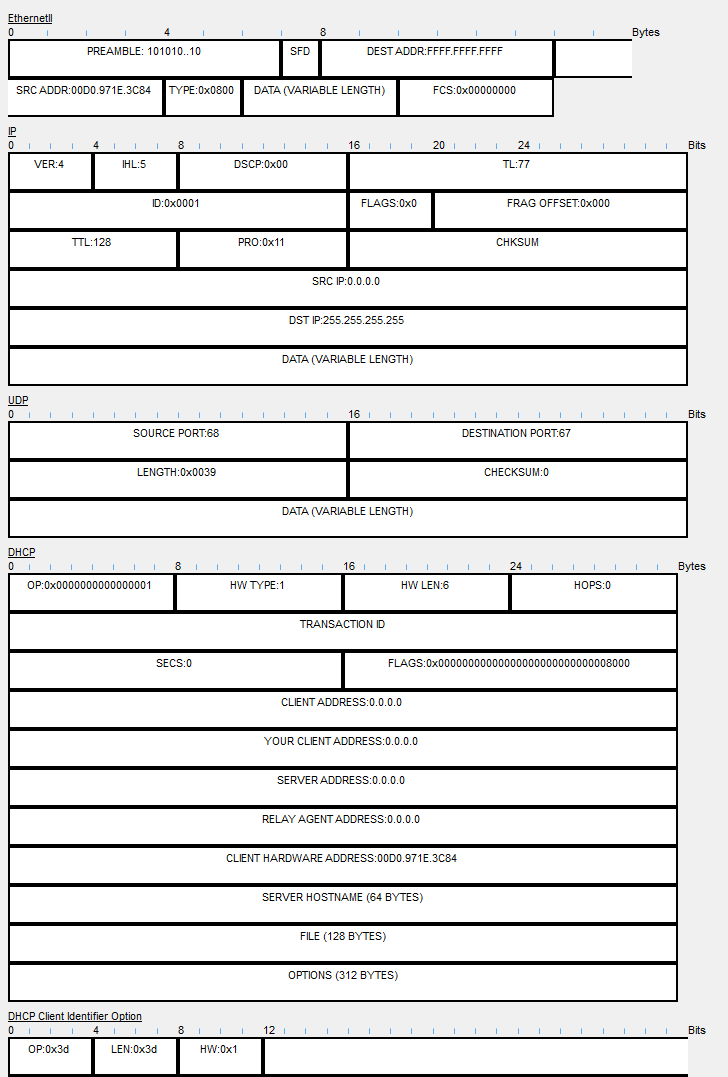
\includegraphics[width=\linewidth, height=0.55\textheight, keepaspectratio]{photos/5-5}
		\caption{DHCP discover message.}
	\end{figure}
	From the above, the following can be noted:
	\begin{itemize}
		\item IP addresses set in DHCP section: Client address, server address, relay agent address
		\item Source port: 68
		\item Destination port: 67
		\item Destination IP address: 255.255.255.255
		\item Destination MAC address: FFFF.FFFF.FFFF
	\end{itemize}
	
	
	Then, Capture then forward is clicked until the DHCP offer message is generated.
	\begin{figure}[H]
		\centering
		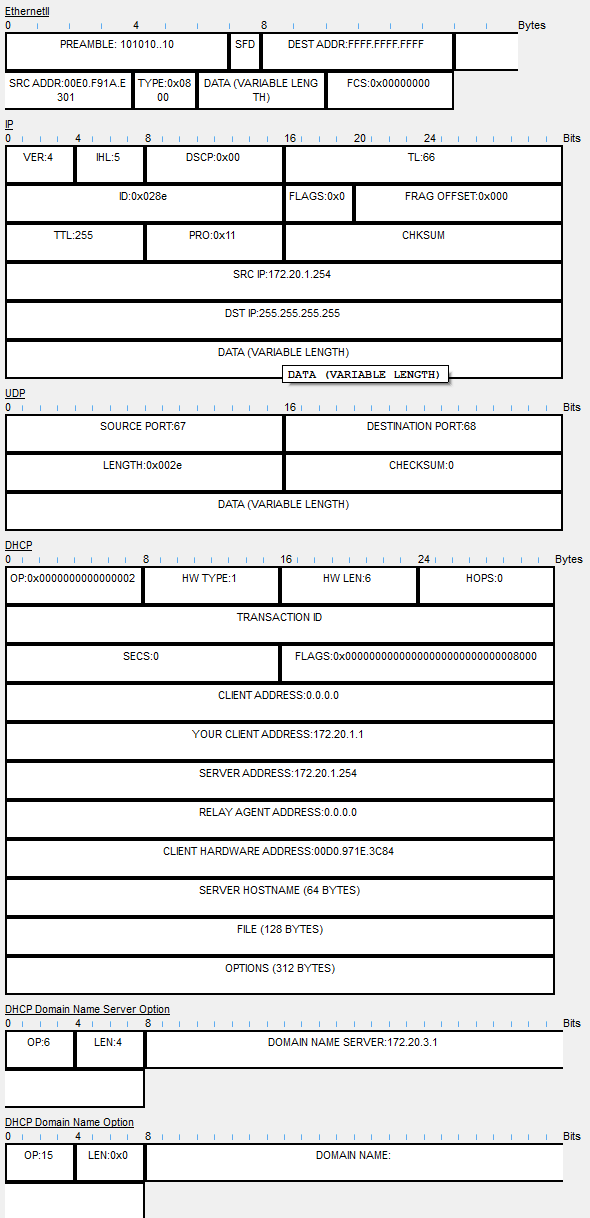
\includegraphics[width=\linewidth, height=0.55\textheight, keepaspectratio]{photos/5-6}
		\caption{DHCP offer message.}
	\end{figure}
	From the above, the following can be noted:
	\begin{itemize}
		\item Pool used to assign the IP configuration: CLIENT-NETWORK
		\item IP addresses router provides to the client: 172.20.1.1, 0.0.0.0
		\item Source port: 67
		\item Destination port: 68
		\item Destination IP address: 255.255.255.255
		\item Destination MAC address: FFFF.FFFF.FFFF
	\end{itemize}
	
	
	Then, Capture then forward is clicked until the DHCP Request message is generated.
	\begin{figure}[H]
		\centering
		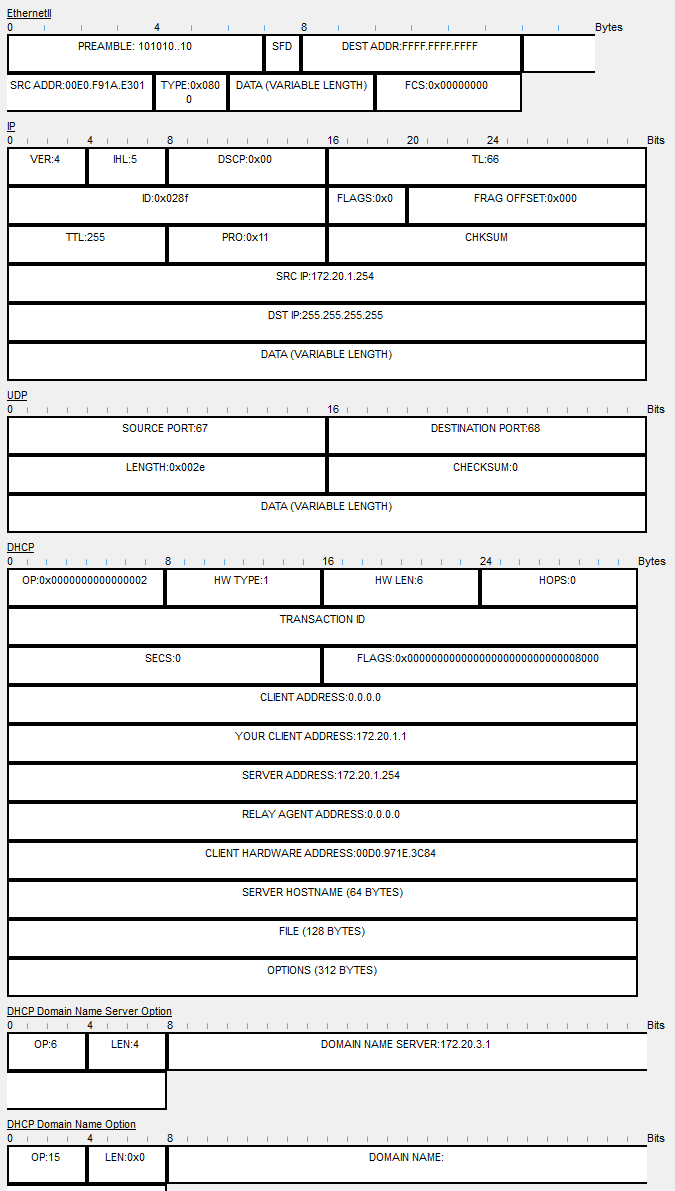
\includegraphics[width=\linewidth, height=0.55\textheight, keepaspectratio]{photos/5-7}
		\caption{DHCP Request message.}
	\end{figure}
	From the above, the following can be noted:
	\begin{itemize}
		\item IP addresses specified by the client: 172.20.1.1, 0.0.0.0
		\item Destination IP address: 255.255.255.255
		\item Destination MAC address: FFFF.FFFF.FFFF
	\end{itemize}
	
	
	Then, Capture then forward is clicked until the DHCP ACK message is generated.
	\begin{figure}[H]
		\centering
		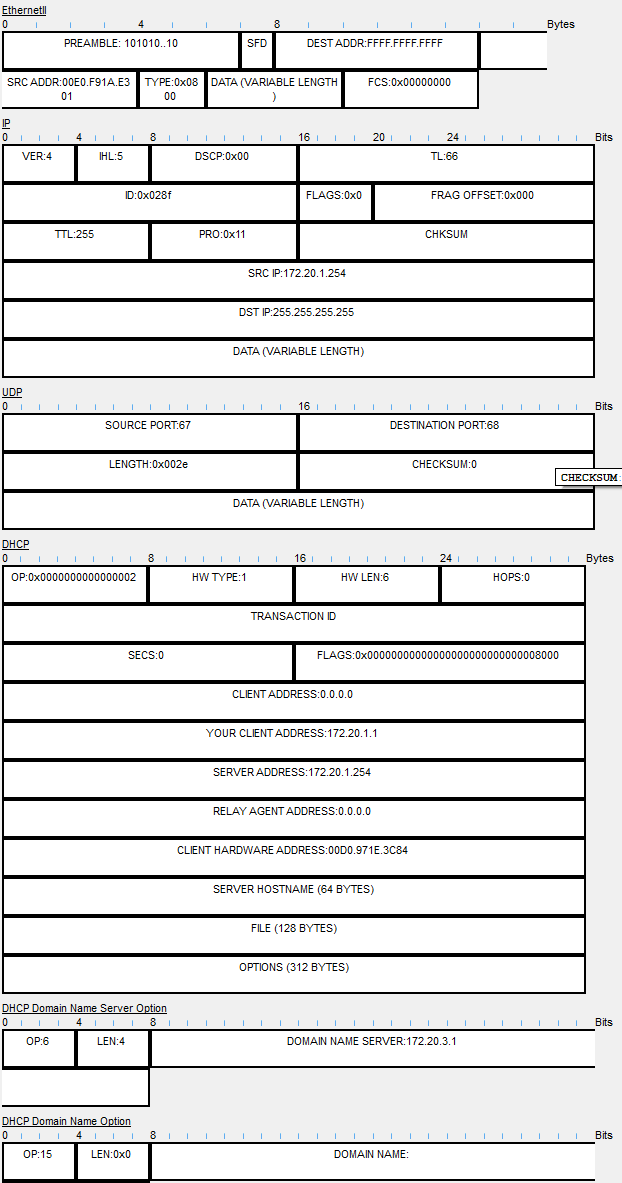
\includegraphics[width=\linewidth, height=0.55\textheight, keepaspectratio]{photos/5-8}
		\caption{DHCP ACK message.}
	\end{figure}
	From the above, the following can be noted:
	\begin{itemize}
		\item How packet content differs from DHCP offer: It does not differ
		\item Destination IP address: 255.255.255.255
		\item Destination MAC address: FFFF.FFFF.FFFF
	\end{itemize}
	
	Capture then forward is clicked until the ACK message reaches the client. This applies the configuration as shown below:
	\begin{figure}[H]
		\centering
		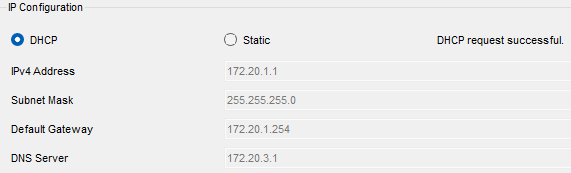
\includegraphics[width=\linewidth, height=0.55\textheight, keepaspectratio]{photos/5-9}
		\caption{Configuration of DHCP client.}
	\end{figure}
	
	To verify the correct configuration, in realtime mode, the server's web page \textit{www.mywebpage.com} is accessed.
	\begin{figure}[H]
		\centering
		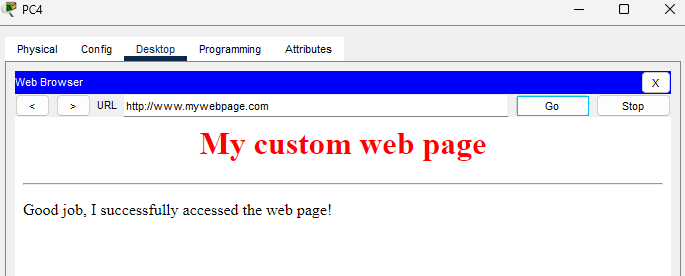
\includegraphics[width=\linewidth, height=0.3\textheight, keepaspectratio]{photos/5-10}
		\caption{\textit{www.mywebpage.com.}}
	\end{figure}
	
	The above process is repeated for the other PC in the same subnet. The IP address it is assigned can be seen below. 
	\begin{figure}[H]
		\centering
		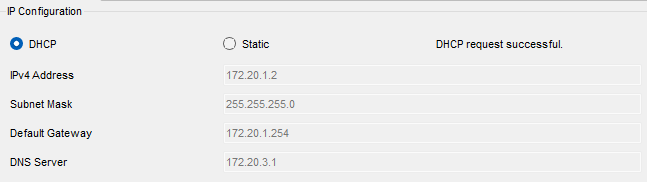
\includegraphics[width=\linewidth, height=0.3\textheight, keepaspectratio]{photos/5-11}
		\caption{Result of DCHP communication on other PC in same subnet.}
	\end{figure}
	
	The above process is repeated for the administrator's PC in the server network. The IP address it is assigned can be seen below. The pool used to choose the address is SERVER-NETWORK.
	\begin{figure}[H]
		\centering
		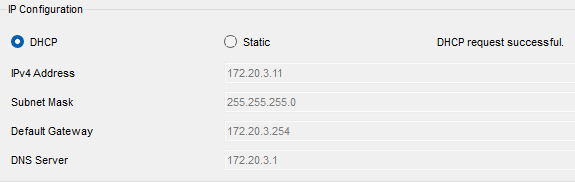
\includegraphics[width=\linewidth, height=0.3\textheight, keepaspectratio]{photos/5-12}
		\caption{Result of DCHP communication on the Administrator's PC.}
	\end{figure}
	
	Finally, in realtime mode, connectivity is verified between the devices as shown below:
	\begin{figure}[H]
		\centering
		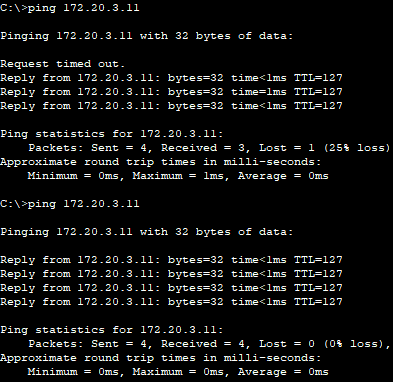
\includegraphics[width=\linewidth, height=0.4\textheight, keepaspectratio]{photos/5-13}
		\caption{Verification of connectivity using ping.}
	\end{figure}
	
	\vspace{1em}
	\hrule
	\vspace{0.5em}
	
	\section*{6. Objective 6}
	
	\textbf{Task Assignment:} The aim of this task was to enable DHCP service on the LAN server and configure R2 as the DHCP relay agent. Additionally, the IP configuration was released and renewed via DHCP and the role of the relay agent was explored.
	
	\textbf{Solution:}\\[1em]
	Before anything else is done, DHCP service on the R2 router is disabled using the \texttt{no service dhcp} command in Configuration mode. This preserves the service while turning it off. This change was verified by switching the administrator's PC configuration to Static and back to dynamic. The result is the following: 
	\begin{figure}[H]
		\centering
		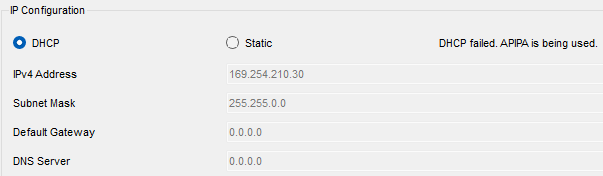
\includegraphics[width=\linewidth, height=0.3\textheight, keepaspectratio]{photos/6-1}
		\caption{New IP address assignment to administrator PC.}
	\end{figure}
	
	After, the service is configured on the Server device. Pools are created for both the server network and the client network.
	\begin{figure}[H]
		\centering
		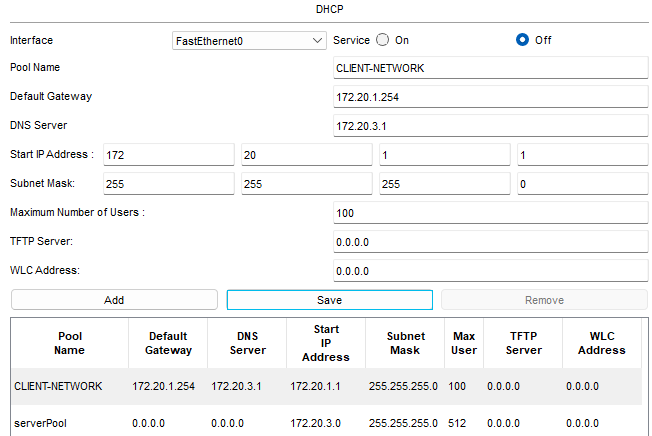
\includegraphics[width=\linewidth, height=0.35\textheight, keepaspectratio]{photos/6-2}
		\caption{Client-Network Pool setup.}
	\end{figure}
	\begin{figure}[H]
		\centering
		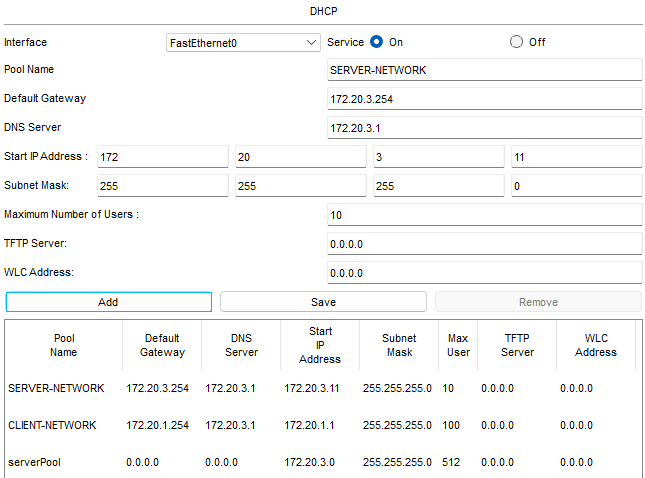
\includegraphics[width=\linewidth, height=0.35\textheight, keepaspectratio]{photos/6-3}
		\caption{Server-Network Pool setup.}
	\end{figure}
	
	Then, on the administrator's PC, the IP configuration is set to Static and then back to dynamic. It then receives the first host address specified in the pool, as shown below:
	\begin{figure}[H]
		\centering
		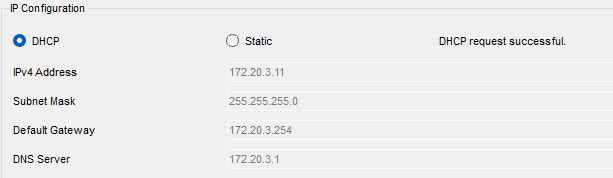
\includegraphics[width=\linewidth, height=0.3\textheight, keepaspectratio]{photos/6-4}
		\caption{Administrator PC receiving first host address specified in the pool.}
	\end{figure}
	
	DHCP configuration is reloaded on the PCs in the client network in the same way. 
	\begin{figure}[H]
		\centering
		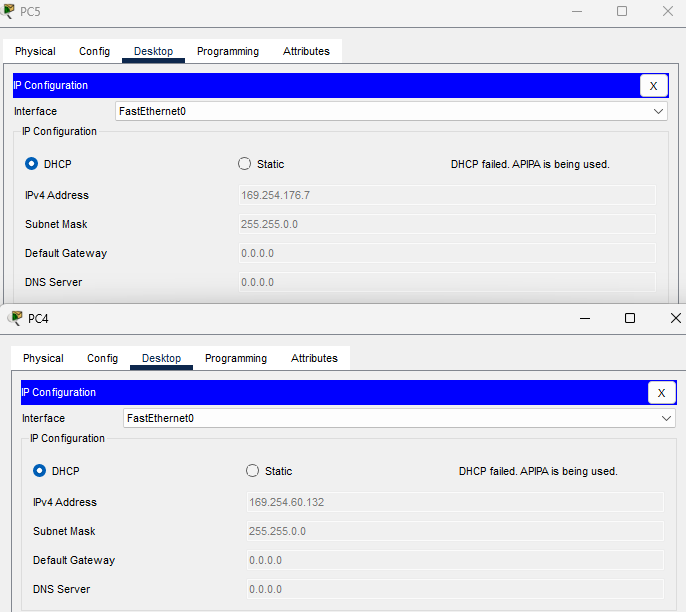
\includegraphics[width=\linewidth, height=0.55\textheight, keepaspectratio]{photos/6-5}
		\caption{DHCP configuration reloaded on the PCs in the client network.}
	\end{figure}
	The PCs received addresses from the APIPA range, this is because currently the only DHCP server is in the different network. It is for this reason that the router is now to be configured to the role of the DHCP relay agent.
	
	After this is done using the commands below, the router is now capable of forwarding DHCP messages arriving at the FastEthernet 0/0 interface to the DHCP server with 172.20.3.1 address.
	\begin{itemize}
		\item \texttt{R2(config)\#interface FastEthernet0/0}
		\item \texttt{R2(config-if)\#ip helper-address 172.20.3.1}
	\end{itemize}
	
	
	
	
	
	
	
	
	After switching to simulation mode, and enabling one PC from the client-network to obtain the DHCP configuration, the DHCP discover message is generated. Capture then forward is clicked until the packet reaches the router.
	
	\begin{figure}[H]
		\centering
		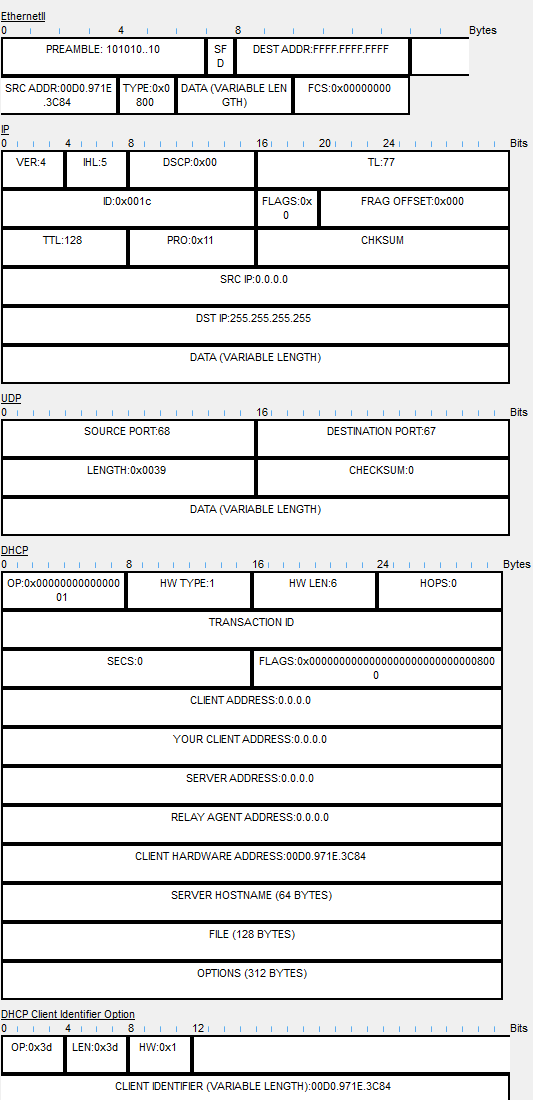
\includegraphics[width=\linewidth, height=0.55\textheight, keepaspectratio]{photos/6-7-in}
		\caption{DHCP discover message at router: Inbound PDU details.}
	\end{figure}
	\begin{figure}[H]
		\centering
		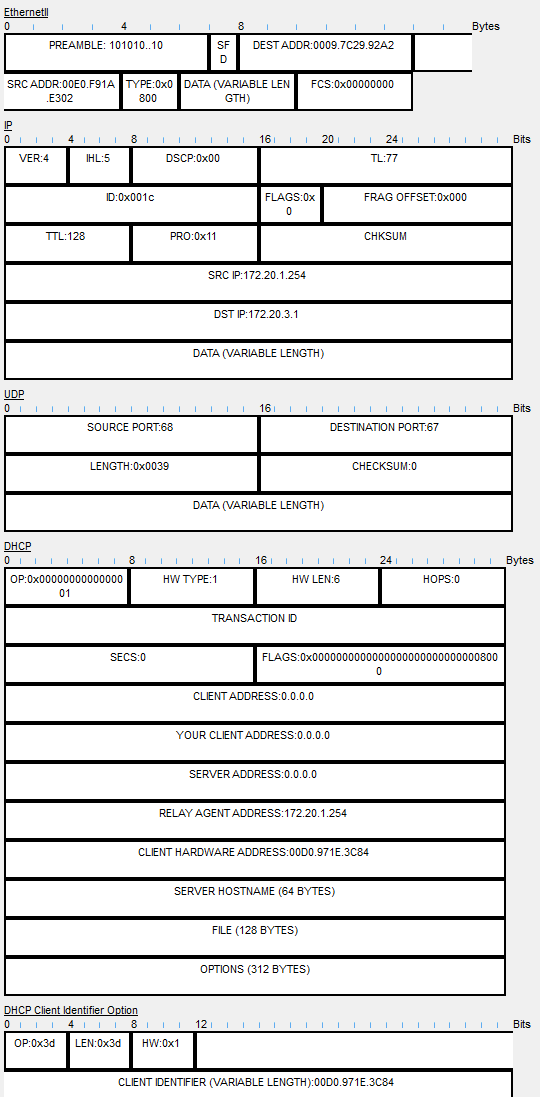
\includegraphics[width=\linewidth, height=0.55\textheight, keepaspectratio]{photos/6-7-out}
		\caption{DHCP discover message at router: Outbound PDU details.}
	\end{figure}
	From the above, the following can be noted:
	\begin{itemize}
		\item Changes in the DHCP section: relay agent address in outbound is not 0.0.0.0
		\item Source MAC address (inbound): 00D0.971E.3C84
		\item Source MAC address (outbound): 00E0.F91A.E302
		\item Destination MAC address (inbound): FFFF.FFFF.FFF
		\item Destination MAC address (outbound): 0009.7C29.92A2
		\item Source IP address (inbound): 0.0.0.0
		\item Source IP address (outbound): 172.20.1.254
		\item Destination IP address (inbound): 255.255.255.255
		\item Destination IP address (outbound): 172.20.3.1
	\end{itemize}
	
	
	Then, Capture then forward is clicked until the DHCP discover message reaches the server
	\begin{figure}[H]
		\centering
		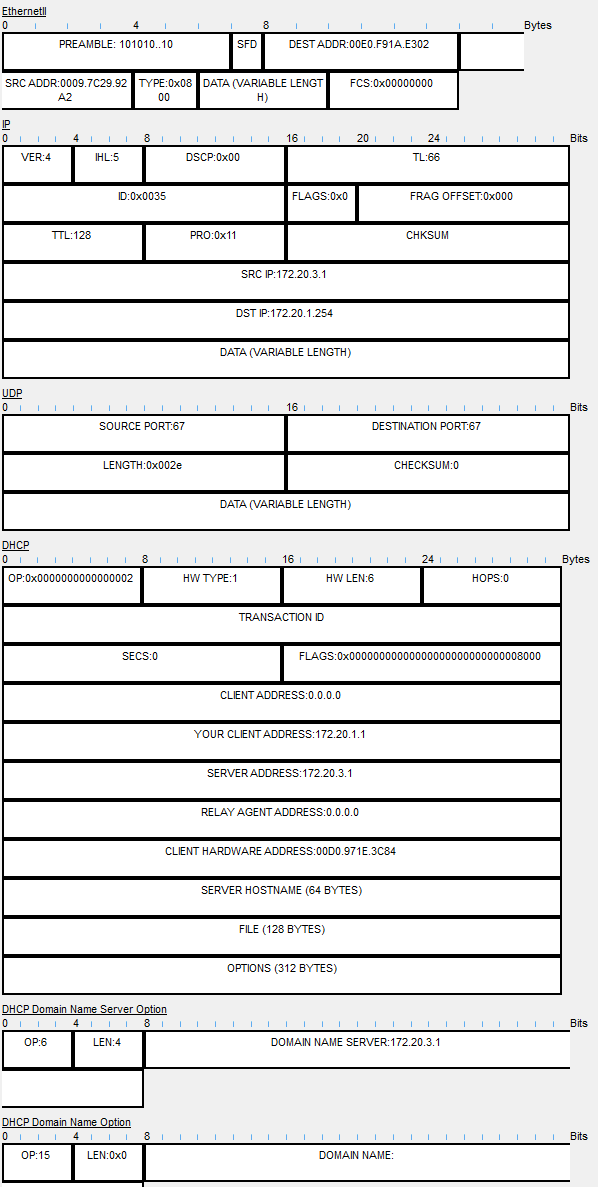
\includegraphics[width=\linewidth, height=0.55\textheight, keepaspectratio]{photos/6-8}
		\caption{DHCP discover message at server.}
	\end{figure}
	From the above, the following can be noted:
	\begin{itemize}
		\item IP addresses included in DHCP section: your client (172.20.1.1), server address (172.20.3.1)
		\item Destination IP address: 172.20.1.254
		\item Destination MAC address: 00E0.F91A.E302
	\end{itemize}
	
	
	Then, Capture then forward is clicked until the DHCP offer message reaches the router.
	\begin{figure}[H]
		\centering
		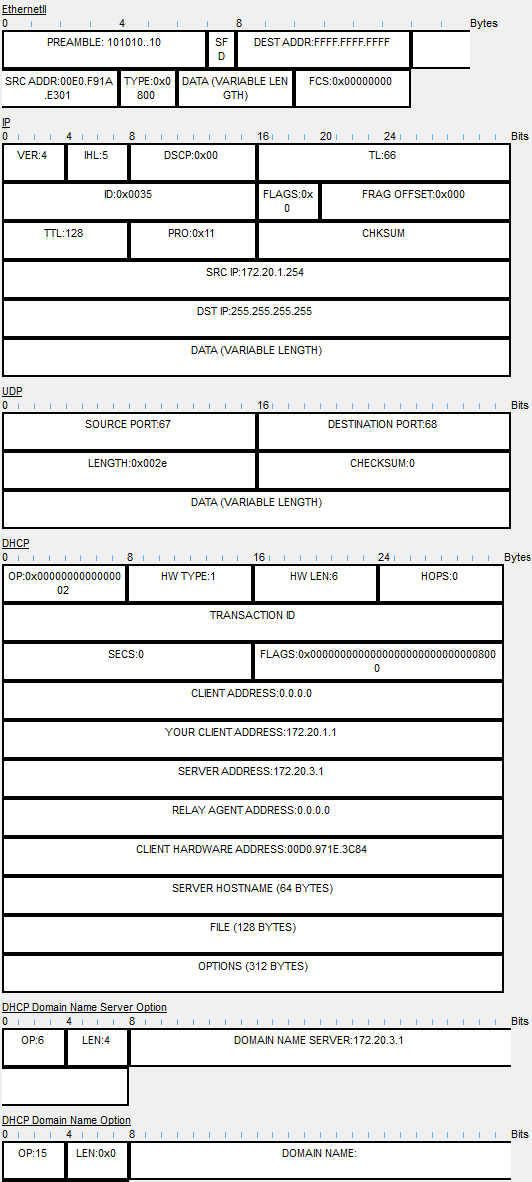
\includegraphics[width=\linewidth, height=0.55\textheight, keepaspectratio]{photos/6-9-out}
		\caption{DHCP offer message at router.}
	\end{figure}
	From the above, the following can be noted:
	\begin{itemize}
		\item Changes in the DHCP section: no changes between inbound and outbound
		\item Source MAC address (inbound): 0009.7C29.92A2
		\item Source MAC address (outbound): 00E0.F91A.E302
		\item Destination MAC address (inbound): 00E0.F91A.E302
		\item Destination MAC address (outbound): FFFF.FFFF.FFFF
		\item Source IP address (inbound): 172.20.3.1
		\item Source IP address (outbound): 172.20.1.254
		\item Destination IP address (inbound): 172.20.1.254
		\item Destination IP address (outbound): 255.255.255.255
	\end{itemize}
	
	
	Then, Capture then forward is clicked until the DHCP offer message reaches the PC and a request message is generated.
	\begin{figure}[H]
		\centering
		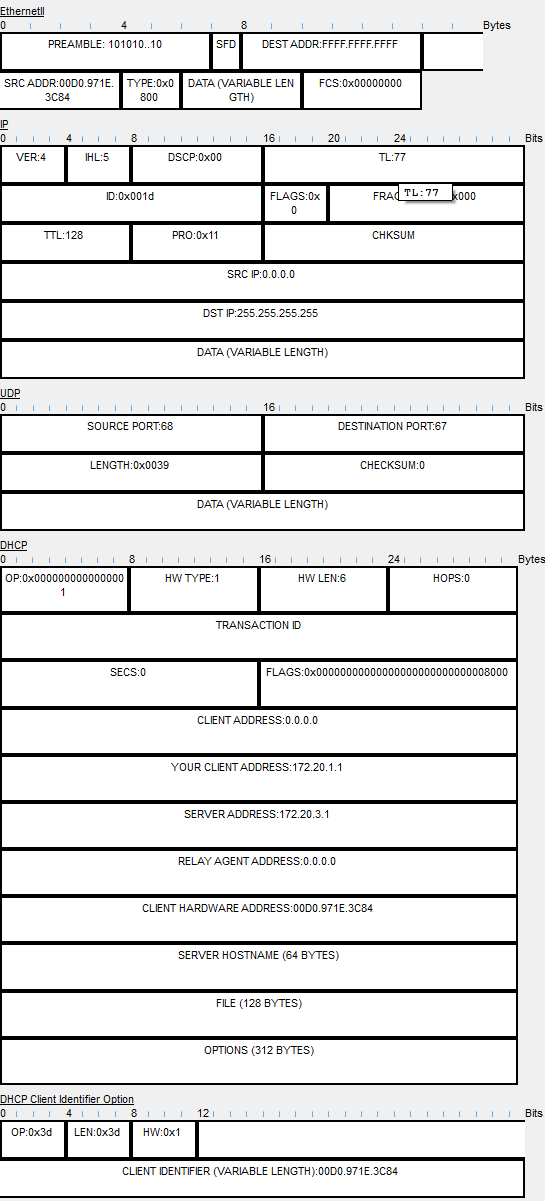
\includegraphics[width=\linewidth, height=0.55\textheight, keepaspectratio]{photos/6-10}
		\caption{DHCP request message generated at PC.}
	\end{figure}
	From the above, the following can be noted:
	\begin{itemize}
		\item How packet content differs from the inbound packet: OP is different (last number 1 instead of 2), and no DHCP domain name area
		\item Destination IP address: 255.255.255.255
		\item Destination MAC address: FFFF.FFFF.FFFF
	\end{itemize}
	
	Then, Capture then forward is clicked until the packet reaches the router once again.
	\begin{figure}[H]
		\centering
		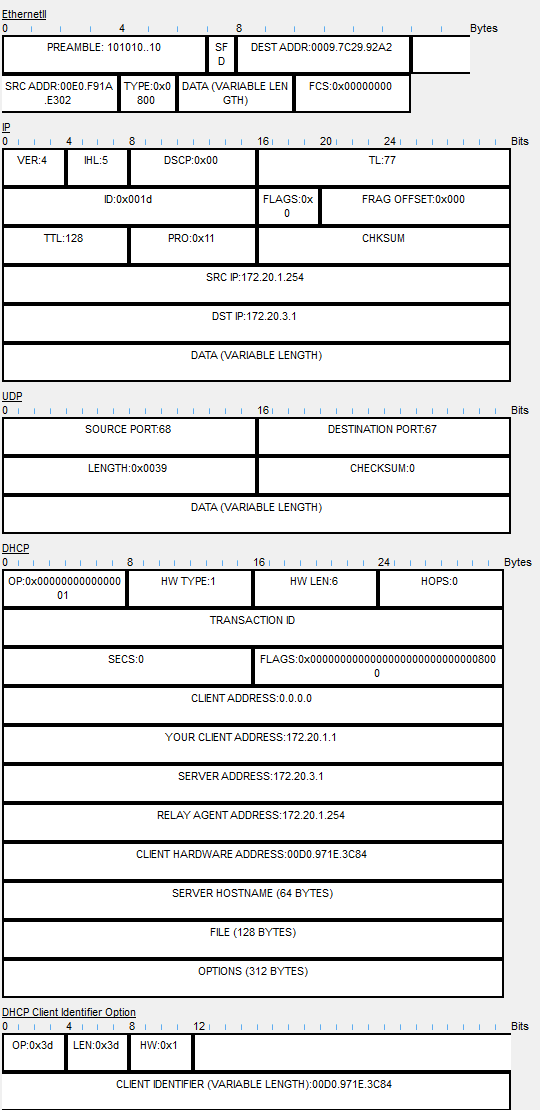
\includegraphics[width=\linewidth, height=0.55\textheight, keepaspectratio]{photos/6-11}
		\caption{DHCP message at the router.}
	\end{figure}
	From the above, the following can be noted:
	\begin{itemize}
		\item How packet content differs from DHCP inbound packeter: The relay agent address is now filled instead of being 0.0.0.0
		\item Destination IP address: 172.20.3.1
		\item Destination MAC address: 0009.7C29.92A2
	\end{itemize}
	
	Then, Capture then forward is clicked until the DHCP message reaches the server and the Ack message is generated.
	\begin{figure}[H]
		\centering
		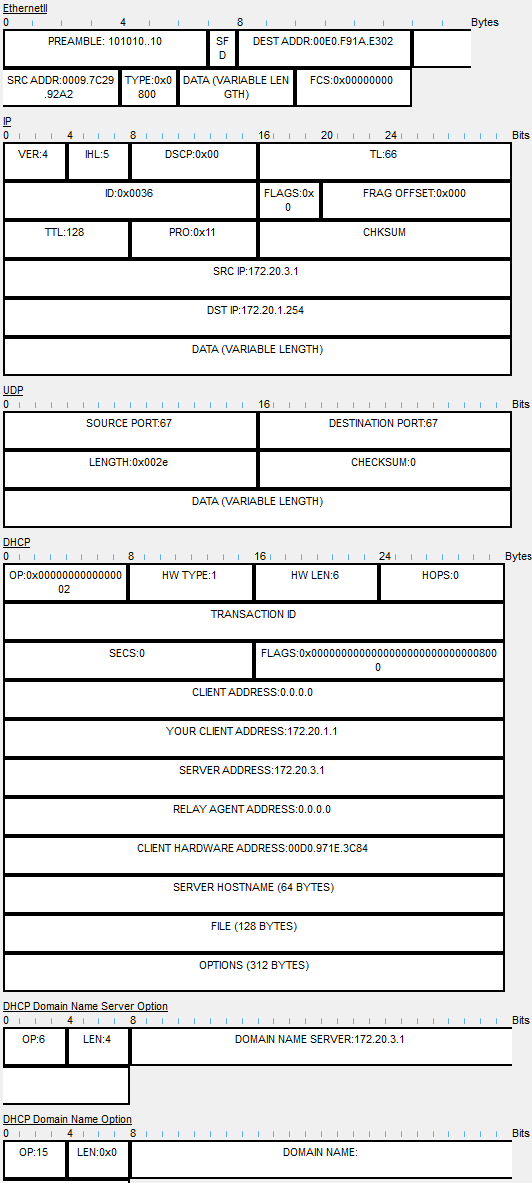
\includegraphics[width=\linewidth, height=0.55\textheight, keepaspectratio]{photos/6-12}
		\caption{DHCP ACK message at the server.}
	\end{figure}
	From the above, the following can be noted:
	\begin{itemize}
		\item How packet content differs from DHCP offer: Although some vaues are different, there are no additional parameters in comparison with the offer
		\item Destination IP address: 172.20.1.254
		\item Destination MAC address: 00E0.F91A.E302
	\end{itemize}
	
	
	Capture then forward is clicked until the DHCP message reaches the router
	\begin{figure}[H]
		\centering
		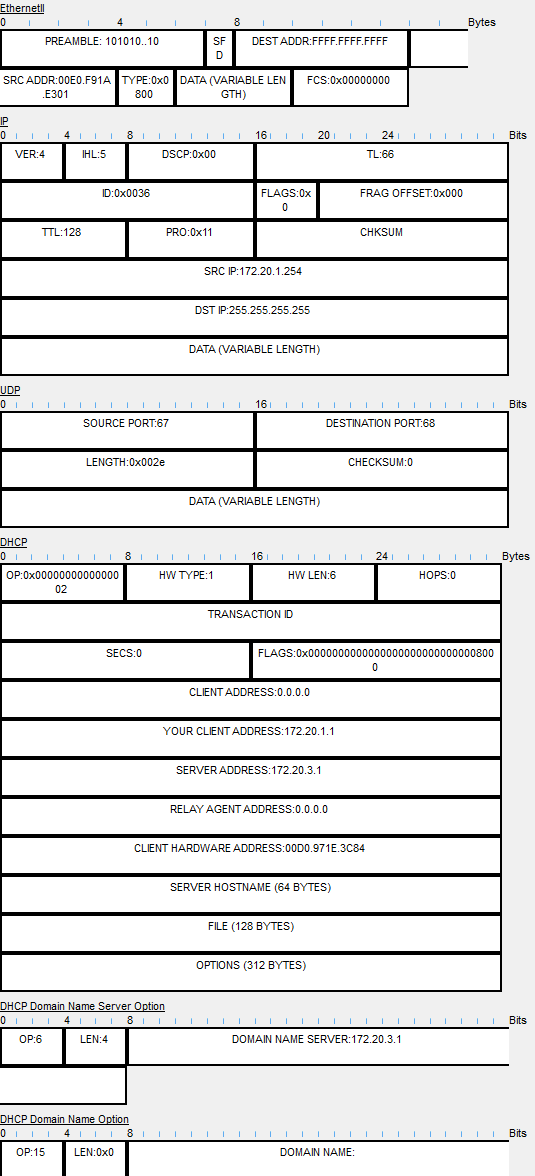
\includegraphics[width=\linewidth, height=0.55\textheight, keepaspectratio]{photos/6-13-router}
		\caption{DHCP message at the router.}
	\end{figure}
	\begin{itemize}
		\item Source MAC address: 00E0.F91A.E301
		\item Destination MAC address: FFFF.FFFF.FFFF
		\item Source IP address: 172.20.1.254
		\item Destination IP address: 255.255.255.255
	\end{itemize}
	
	Finally, capture then forward is clicked until the packet reaches the PC. Realtime mode is enabled, and connectivity is verified by accessing \texttt{www.mywebpage.com}. The configuration set and the accessing of the webpage are shown below.
	
	\begin{figure}[H]
		\centering
		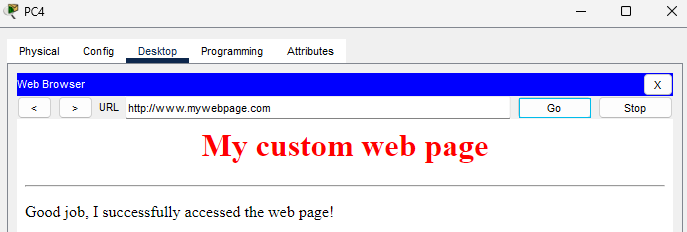
\includegraphics[width=\linewidth, height=0.55\textheight, keepaspectratio]{photos/6-13-page}
		\caption{Website successfully accessed.}
	\end{figure}
	\begin{figure}[H]
		\centering
		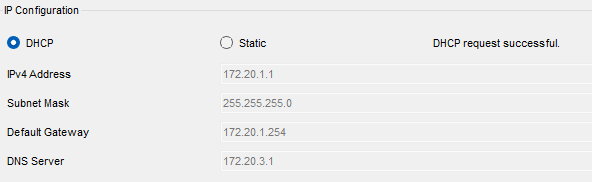
\includegraphics[width=\linewidth, height=0.55\textheight, keepaspectratio]{photos/6-13-pc}
		\caption{Current configuration of the PC.}
	\end{figure}
	
	The IP address of the other PC in the same subnet is as shown below. 
	\begin{figure}[H]
		\centering
		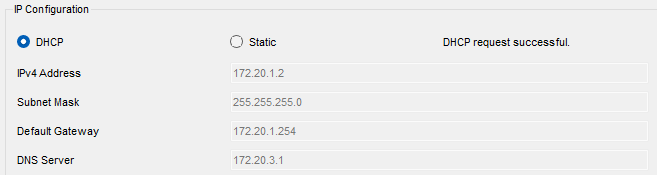
\includegraphics[width=\linewidth, height=0.55\textheight, keepaspectratio]{photos/6-14}
		\caption{IP address of the other PC in the same subnet.}
	\end{figure}
	
	Connectivity is finally verified between other devices via ping
	\begin{figure}[H]
		\centering
		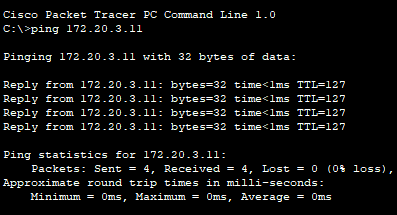
\includegraphics[width=\linewidth, height=0.4\textheight, keepaspectratio]{photos/6-15}
		\caption{Successful connectivity verification via ping.}
	\end{figure}

	
	\vspace{1em}
	\hrule
	\vspace{0.5em}
		
	\section*{7. Final Questions}
	
	
	\textbf{Question 1: How many messages are exchanged during the initial address assignment? What are they called?}\\
	The initial DHCP address assignment consists of \textbf{four} messages.
	\begin{itemize}
		\item \textbf{DHCP Discover:} sent by the client to locate available DHCP servers
		\item \textbf{DHCP Offer:} sent by the server offering an IP address and configuration
		\item \textbf{DHCP Request:} sent by the client to request the offered IP address
		\item \textbf{DHCP Acknowledgment (ACK):} sent by the server to confirm the address assignment
	\end{itemize}
	
	\textbf{Question 2: What is defined by the lease time?}\\
	The lease time defines:
	\begin{itemize}
		\item The duration for which an IP address is valid and assigned to a client
		\item The time after which the client must renew the lease or release the address back to the DHCP server
	\end{itemize}
	
	\textbf{Question 3: What is the relay agent used for?}\\
	A DHCP relay agent is used to forward DHCP messages between clients and servers located on different networks
	
	\textbf{Question 4: When a relay agent is used in the DHCP communication, how does a server identify which pool to use to assign the address?}\\
	The DHCP server identifies the correct address pool by:
	\begin{itemize}
		\item Examining the Gateway IP address field
		\item Using the Gateway IP address value to determine the subnet of the requesting client and selecting the appropriate DHCP pool
	\end{itemize}
	
	\textbf{Question 5: How does a relay agent alter destination IP and MAC addresses while forwarding the DHCP messages?}\\
	When forwarding DHCP messages, the relay agent:
	\begin{itemize}
		\item Changes the \textbf{destination IP address} from the broadcast address to the DHCP server’s unicast IP address
		\item Updates the \textbf{destination MAC address} to the MAC address of the next-hop device toward the server
		\item Inserts its own IP address into the Gateway IP address field before forwarding the message
	\end{itemize}
	
	\vspace{1em}
	\hrule
	\vspace{0.5em}
	
\end{document}
